\documentclass[../main.tex]{subfiles}
\begin{document}
	$G(A_1\ldots a_k) = ((a_i, a_j))_{k\times k}$\n
	$g(a_1 \ldots a_k) = det\ G = || b_1||^2 \ldots || b_k || ^2$\n
	$
	a_1 \ldots a_k \underset{\text{Г-Ш}}{\leadsto} \underset{\text{попарно-ортог}}{b_1 - b_k}$\n
	\begin{minipage}{150px}
		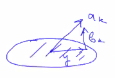
\includegraphics[width=150px]{pic05}
	\end{minipage}	
	\begin{minipage}{\textwidth-150px}
		$L = span(a_1 \ldots a_{k-1}) = span(b_1 \ldots b_{k-1})$\n
		$a_k = y + b_k$\n
		$b_k - $ ортогон. сост. $a_k$ относит. $L$
	\end{minipage}
	\begin{defin}
		$(V, (\cdot, \cdot)) \; \; a_1 \ldots a_k \in V \; \; \; \; \; \; 1\leq k \leq n$\n
		$\prod (a_1 \ldots a_k) = \{x \in V | x = \sum\limits_{i=1}^k
		\alpha_i a_i \; \; \underset{\forall i = 1, k}{\alpha_i \in [0, 1]}\}$\n
		$k$-мерный параллелепипед, построенный на векторах $a_1 \ldots a_k$
	\end{defin}
		$V = V_3 \cong \R^3 \\
		k = 1 \; \; \; x = \alpha_1 a_1 \; \; \; \alpha_1 \in [0, 1] \; \; \; 0 \longrightarrow a_1 \; \; \text{отрезок}\\
		k = 2 \; \;$ 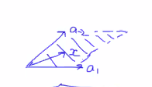
\includegraphics[width=130px]{pic06}$\; \;\begin{matrix}
			 x = \alpha_1 a_1 + \alpha_2 a_2 \\
			\alpha_{1, 2} \in [0, 1]
		\end{matrix} \; \; \; \text{параллелограмм}\\
		k = 3 \; \; $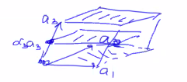
\includegraphics[width=130px]{pic07} $\; \; \; \begin{matrix}
			x = \alpha_1 a _1 + \alpha_2 a_2 + \alpha_3 a_3 \\
			\alpha_i \in [0, 1]
		\end{matrix} \; \; \text{параллелиипед}$
	\begin{defin}
			$V(\prod(a_1 \ldots
			 a_k)) = (g ( a_1 \ldots a_k))^{1/2} \text{ объем к-мерного пар-да}$\n
			 $\boxed{V ( \prod(a_1 \ldots a_k )) = V ( \prod(a_{1}\ldots a_{k-1})) \cdot || b_k ||} \; \; \text{см. следствие к т-ме о det G}\\
			 a_1 \ldots a_k \underset{\text{Г-Ш}}{\leadsto} b_1 \ldots b_k$\n
	\end{defin}
	\begin{mylist}
		\item 
		$k = 1 \; \; \; V(\longrightarrow a_1) = \sqrt{g(a_1)} = \sqrt{(a_1, a_1)} = ||a_1 || \text{ -- длина отрезка}$
		\item 
		$k = 2 \; \; \; V($\belowbaseline[-40pt]{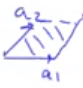
\includegraphics[width=50px]{pic08}}  $) = \sqrt{g(a_1, a_2)} = \sqrt{g(a_1)} \cdot \| b_2 \| = \|a_1\| \cdot \|b_2\| = \underset{\text{ основание   высота}}{||b_1|| \cdot || b_k ||} = S \text{ площадь пар.}\\$
		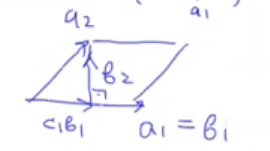
\includegraphics[width=100px]{pic09}
		\item $
		k = 3 \; \;
		$\belowbaseline[-30pt]{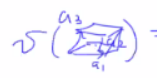
\includegraphics[width=80px]{pic10}}$ \;  = \sqrt{g(a_1, a_2, a_3)} =\begin{matrix}
			\| b_1\| \|b_2\|\\
			||\\
			\sqrt{g(a_1, a_2)}\\
			||\\
			S \text{ основания}
		\end{matrix} \cdot \begin{matrix}
			\\\\
			||b_3||\\
			||\\
			h \text{ высота}
		\end{matrix} = V_\text{пар-да}
		$\\
		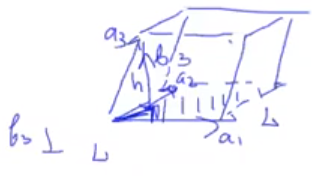
\includegraphics[width=130px]{pic11}
	\end{mylist}
	$a_1 \ldots a_k \text{ линейно зав.} \Leftrightarrow g(a_1 \ldots a_k) = 0\\
	k = 2 \; \; \; a_1, a_2 \text{ коллин. } \Leftrightarrow S_\text{пар.} = 0\\
	k = 3 \; \; \; a_1 a_2 a_3 \ \; \text{ компл. } \Leftrightarrow V = 0$
	\n
	\newpage
	$\pu e_1 \ldots e_n$ базис $V \; \; \; \; \; \; \; \; \; \Gamma = ((e_i, e_j)) = G(e_1 \ldots e_n)$
	\n
	\textbf{Свойства $\Gamma$}
	\begin{mylist}
		\item 
		$\Gamma^* = \Gamma$ (самосопряженность)
		\item $\forall x \neq 0 \; \; \; \; x = \sum\limits_{i=1}^n x_i e_i \; \; \; \; \; \underset{=(x, x)}{\lambda^T \Gamma \  \vec x} > 0$\n
		Эти 2 свойства = $\boxed{\Gamma > 0}$ \underline{Положительно определенная матрица}
		\item $\triangle_k  = g(e_1 \ldots e_k)$ угловые миноры матрицы $\Gamma$\n
		$\Gamma = \left(\begin{array}{c|c|c|c}
			(e_1, e_1) & (e_1, e_2) & (e_1, e_3) & \ldots\\
			\cline{1-1}
			\novline{1}{
				(e_2, e_1)} &  (e_2, e_2)
			 & (e_2, e_3) & \ldots\\
		\cline{1-2}
		\novline{1}{(e_3, e_1)}
		& \novline{1}{(e_3, e_2)}
		& (e_3, e_3)
		& \ldots\\
		\cline{1-3}
		\novline{4}{\ldots}
		\end{array}\right) \; \; \; 
		\boxed{\forall k = 1 \ldots n \; \; \; \triangle_k > 0}$
		\begin{proof}
			Из следствия 1 $a_1 \ldots a_k$ лин. независ. $\Leftrightarrow g(a_1 \ldots a_k) > 0\\
			e_1 \ldots e_k$ лин. независ. $\forall k = 1 \ldots n$
		\end{proof}
		В частности $\triangle_n = det \ \Gamma > 0 \Rightarrow$ \underline{$\Gamma$ невырождена}
		\item 
		$\begin{matrix}
			e_1 \ldots e_n\\
			e'_1 \ldots e'_n
		\end{matrix}$ базисы $V \; \; \; \; \begin{matrix}
			T = T_{e\rightarrow e'}\\
			\boxed{\Gamma' = T^T \ \Gamma \ \vec T}
		\end{matrix} \; \; \Gamma = ((e_i, e_j)) \; \; \; \Gamma' = ((e'_i, e'_j))$
		\begin{proof}\ \\
			$x \leftrightarrow x$ в базисе $e\n
			\leftrightarrow x' $ в базисе $e'\; \; \; \; \; \; \; \; \;
			x = Tx'\n
			(x, y) = x^T \Gamma \vec y = (x')^T T^T \Gamma \vec T \vec y'\\
			||\\
			(x')^T \Gamma' \vec y'\n
			\forall x, y \; \; \; x = e'_i \; \; \; y = e'_j\n
			\boxed{\Gamma' = T^T \Gamma \vec T}$
		\end{proof}
		В частности, $e$ и $e'$ о.н.б. $V \; \; \; \; \Gamma = \Gamma' = E\n
		E = T^T \vec T \Rightarrow \underbrace{\vec{T^T}}_{T^*} T = E \; \; \; \boxed{T^* T = E}\n
		\boxed{e, e' \text{ о.н.б.} \Rightarrow  T = T_{e\rightarrow e} \text{ унитарн.(ортог.)}}$
	\end{mylist}
	\begin{defin}
		\underline{Невырожд.} комплекснозн. (веществ) матрица $Q_{n\times n}$ называется\\ \underline{унитарной (ортогональной)}, если $Q^* = Q^{-1} ( \Leftrightarrow Q^* Q = Q Q^* = E)$
	\end{defin}
	\textbf{Свойства унитарной (ортог.) матрицы}
	\begin{mylist}
		\item 
		$Q \text{ унитарн. (ортогог.)} \Leftrightarrow \text{стр. (столб) попарно-ортагон. (в смысле станд. скал. про-я}\\
		\text{ в пр-ве } \R^n (\mathbb{C}^n) \; \; \; (x, y) = \sum\limits_{i=1} ^ n x_i y_i)$
		\begin{proof}
			$Q = (Q_1 \ldots Q_n) \text{столбцы}\\
			Q\text{ унит. (ортог.)} \Leftrightarrow Q^* = Q^{-1} \Leftrightarrow Q^* = \vec{Q^T} = \begin{pmatrix}
				\vec{Q_1^T}\\
				\vdots\\
				\vec{Q^T_n}
			\end{pmatrix}$\n
			$Q^* Q = E$\n
			$E = Q^* Q = \begin{pmatrix}
				\vec{Q}^T_1 Q_1 & \vec Q^T_1 Q_2 & \vec Q^T_1 Q_n\\
				\ldots\\
				\vec Q^T_n Q_1 &\vec Q^T_n Q_2 & \vec Q^T_n Q_n
			\end{pmatrix} = 
			((\vec{Q_i, Q_j})) \leftrightarrow (Q_i, Q_j) = \delta_{i j} \text{ аналогично для строк}
			$
		\end{proof}
		\item 
		$|detQ| = 1$
		\begin{proof}
			$1 = det E = det(Q^* Q) = \begin{matrix}
			det(Q^*)\\
			||\\
			\vec{Q^T}
			\end{matrix} \cdot det \ Q = \vec{det \ Q}\cdot det\ Q = |det Q| ^2$
		\end{proof}
		$\boxed{\text{евкл.:} \; Q_{\text{ортогон.}} \rightarrow det Q = \pm1}$\\
	\item 
	$Q^{-1} - \text{ унитарн.(ортогон.)}$
	\begin{proof}
		$(Q^{-1})^* = \vec{(Q^{-1})^T} = (\vec{Q^T})^{-1} = (Q^*)^{-1} = Q = (Q^{-1})^{-1}$
	\end{proof}	
	\item $Q, R$ унитарн.(ортог.) $\Rightarrow QR$ унит. (ортогон.)
	\begin{proof}
		$(QR)^* = (\vec{QR})^T = \vec R^T \vec Q^T = R^* Q^* = R^{-1} Q^{-1} = (QR)^{-1}$
	\end{proof}
	\item $\begin{matrix}
		e, e' \text{ о.н.б.} V\\
		T = T_{e\rightarrow e'}
	\end{matrix} \Rightarrow T$ -- унитарн.(ортог.) матрица.
	\begin{examples}
		Матрицы поворота на плоскости или в пространстве\n
		$T = \begin{pmatrix}
			\cos \alpha & - \sin \alpha\\
			\sin \alpha & \cos \alpha
		\end{pmatrix}$ ортогональна.
	\end{examples}
	\end{mylist}

	\subsection{Ортогональное дополнение. Задача о перпендикуляре. Теорема Пифагора. Теорема о наилучшем приближении. Тождество Парсеваля. Неравенство Бесселя.}
	\begin{defin}
		$\underset{\text{лин. подпр.}}{L\subset V} \; \; \; L^\perp = \{ y \in V |\  \forall x \in L (x, y) = 0\}\\
		\text{ -- \underline{ ортогональое дополнение подпро-ва }L}$
	\end{defin}
	\textbf{Свойства $L^\perp$}
	\begin{mylist}
		\item 
		$L^\perp \text{ линейное подпро-во}$
		\begin{proof}
			$\forall \lambda \in K, \; \forall u, v \in L^\perp : \forall x \in L(x, u) = 0, (x, v) = 0\n
			(x, u + \lambda v) = \underset{= 0}{(x, u)} + \vec \lambda \underset{= 0}{(x, v)} = 0 \Rightarrow u + \lambda
			 v \in L^\perp$
		\end{proof}
		\item 
		$\boxed{V = L \bigoplus L^\perp}$
		\begin{proof}
			$L = span\underset{\text{лин. незав. н.у.о. попарно ортогон. (Г-Ш)}}{(a_1 \ldots a_k)}\n
			a_1 \ldots a_k \underbrace{a_{k+1} \ldots a_n}\\
			\text{дополним до базиса } V \text{ н.у.о. попарно ортогон. (Г-Ш)}\n
			L^{\perp ?} = span(a_{k+1} \ldots a_n) \; \; \; V = L \bigoplus L^\perp\n
			\forall x \in L: \; \; x = \sum\limits_{i=1}^k c_i a_i \n
			\forall y \in L^\perp: \; \; y \ \sum\limits_{j = k+1}^n c_j a_j \n
			(x, y) = \sum\limits_{i=1}^k \sum\limits_{j = k+1}^n c_i \vec c_j \underset{=0}{(a_i, a_j)} = 0 \Rightarrow L^\perp$ -- ортогон. дополн. $L$
		\end{proof}
	\item 
	$(L^\perp)^\perp = L$
	\begin{proof}
		$\forall x \in L \; \; \forall y \in L^\perp : (x, y) = 0 \; \n
		\Rightarrow L \subset (L^\perp)^\perp \n
		(L^\perp)^\perp \oplus L^\perp = V = L \oplus L^\perp \n
		\Rightarrow dim (L^\perp)^\perp = dim L \Rightarrow L = (L^\perp)^\perp$
	\end{proof}
	\item 
	$(L_1 + L_2)^\perp = L_1^\perp \cap L_2^\perp\n
	(L_1 \cap L_2)^\perp = L_1^\perp + L_2^\perp \n
	\text{Похоже на правило Де Моргана, но не то же самое}$
	\begin{proof}
		$(L_1 + L_2)^\perp = L_1^\perp \cap L_2 ^ \perp\n
		\begin{matrix}
		\forall x \in L_1 + L_2\\
		||\\
		l_1 + l_2\\
		\in L_1 \; \in L_2
		\end{matrix} \; \; \forall y \in (L_1 + L_2)^\perp \; \; 
		\begin{matrix}
			(x, y) = 0\\
			||\\
			(l_1, y) + (l_2, y)
		\end{matrix}\n
		\left.\begin{array}{c}
		\pu l_2 = 0 \; \; \underset{\forall l_1 \in L_1}{(l_1, y) = 0} \; \Rightarrow y \in L_1^\perp\\
		\pu l_1 = 0 \; \; \underset{\forall l_2 \in L_2}{(l_2, y) = 0} \; \Rightarrow
		 L_2^\perp
		 \end{array}\right\} \Rightarrow y \in L_1 ^\perp \cap L_2 ^\perp$\n
		 $\Rightarrow \boxed{(L_1 + L_2)^\perp \subset L_1^\perp \cap L_2^\perp}$\n
		 \underline{Обратно:}
		 $\pu y \in L_1^\perp \cap L_2^\perp \Rightarrow \begin{matrix}
			 \forall l_1 \in L_1 & (l_1, y) = 0\\
			 \forall l_2 \in L_2 & (l_2, y) = 0
		 \end{matrix} \Rightarrow 
		 \begin{matrix}
			 \forall x = l_1 + l_2 \in L_1 + L_2\\
			 (x, y) = (l_1, y) + (l_2, y) = 0
		 \end{matrix}\n
		 \Rightarrow y \in (L_1 + L_2)^\perp \Rightarrow \boxed{L_1^\perp \cap L_2^\perp \subset (L_1 + L_2)^\perp} \Rightarrow (L_1 \cap L_2)^\perp = L_1 ^ \perp + L_2^\perp\n\n
		 (L_1 \cap L_2)^\perp = L_1^\perp + L_2^\perp\n
		 (L_1^\perp + L_2^\perp)^\perp \underset{\text{по доказ-му}}{=} (L_1^\perp)^\perp \cap (L_2^\perp)^\perp \underset{\text{св-во 3}}{=} L_1 \cap L_2\n
		 \text{св-во 3   } \; L_1^\perp + L_2^\perp = (L_1 \cap L_2)^\perp$
	\end{proof}
	\item 
	$V^\perp = \0\n
	\0^\perp = V$
	\end{mylist}
	\begin{defin}
		$\forall x \in V \; \exists! y \in L, \exists! \ z \in L^\perp : \boxed{x = y+z}$\\
		из св-ва 2\\
		$y$ -- ортогон. проекция $x$ на лин. подпро-во $L$\\
		$z $ -- ортогон. составл. $x$ относительно $L$ -- перпендикуляр, опущенный из $x $ на $L$\\
		$(x, y) = 0$\\
		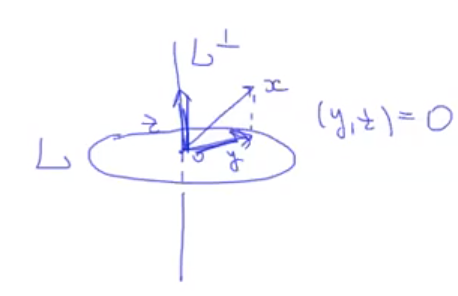
\includegraphics[width=150px]{pic12}\\
	\end{defin}
	\textbf{Задача о перпендикуляре $z = ?$}\n
	$L = span(\underset{\text{лин. независ.}}{a_1 \ldots a_k}) \; \; x \in V \; \; \; x = y+z \; \;
	\; \;  y\in L\; \; \; \; 
	z\in L^\perp \; \; \;  \; \; z = ?\n
	y \in L \; \; \; \; \; 
	y = \sum\limits_{i=1}^k c_i a_i\n
	x = \sum\limits_{i=1}^k c_i a_i + z \; \; \; | \cdot a_j\n
	\forall j = 1\ldots k \; \; \; \; \; \; \; \
	(x_i a_j) = \sum\limits_{i=1}^k c_i (a_i, a_j) + \underset{=0}{(z, a_j) \in L} \underset{z \in L^\perp}{=} \sum\limits_{i=1}^k c_i(a_i, a_j) \; \; \; \; \; \; c_i = ?$\n
	СЛНУ \n
	$
	\underbrace{
	\begin{pmatrix}
	(a_1, a_1) & (a_2, a_1) \ldots\\
	(a_1, a_2) & \ldots\\
	\ldots & \ldots
	\end{pmatrix}}_{G^T(a_1 \ldots a_k)} \begin{pmatrix}
		c_1 \\
		\vdots\\
		c_k
\end{pmatrix} = \begin{pmatrix}
(x, a_1)\\
\vdots\\
	(x, a_k)
\end{pmatrix}\n
	det G > 0 \rightarrow \exists ! \text{ реш-е} c_1 \ldots c_k\n
	\leadsto y = \sum\limits_{i=1}^k c_i a_i \leadsto z = x - y.
	$
	\begin{examples}
		$L = span(a_1 a_2 a_3)$\n
		$a_1 = \begin{pmatrix}
			1\\1\\1\\1
		\end{pmatrix} \; \; 
		a_2 = \begin{pmatrix}
			1\\2\\2\\-1
		\end{pmatrix} \; \; 
		a_3 = \begin{pmatrix}
			1\\0\\0\\3
		\end{pmatrix} \; \; 
		x = \begin{pmatrix}
			4\\-1\\-3\\4
		\end{pmatrix} \; \; z = ?\n
		a_3 = 2a_1 - a_2 \; \; \; L = span(a_1, a_2)\n
		\underset{\text{вещ.}}{G^T} = G = \begin{pmatrix}
			4 & 4\\ 4 & 10
		\end{pmatrix} \; \; \; \begin{matrix}
			(x, a_1) = 4\\
			(x, a_2) = -8
		\end{matrix} \; \; 
		\begin{pmatrix}
			4 & 4 & | & 4\\
			4 & 10 & | &-8
		\end{pmatrix} \leadsto \begin{pmatrix}
			1 & 1 & | & 1\\
			0 & 6 & | & -12
		\end{pmatrix}\n
		c_1 = 3 \; \; c_2 = -2\n
		y = 3a_1 - 2a_2 = \begin{pmatrix}
			1\\-1\\-1\\5
		\end{pmatrix} \; \; z = x-y \ \begin{pmatrix}
			8\\0\\-2\\-1
		\end{pmatrix} \; \; (y, z) = 0$ 
	\end{examples}
	\begin{theorem}[Пифагора]\ \\
		$\forall y, z \in V \; \; (y, z) = 0 \Rightarrow ||y+z||^2 = ||y||^2 + ||z||^2$\\ 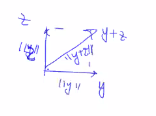
\includegraphics[width=150px]{pic13}
	\end{theorem}
	\begin{proof}
		$||y+z||^2 = (y+z, y+z) = \underset{=||y||^2}{(y, y)} + \underset{= 0}{(y, z)} + \underset{=0}{(z, y)} + \underset{=||z||^2}{(z, z)}$
	\end{proof}
	\begin{corollary}
		$x_1\ldots x_k \text{ попарно-ортог. } \Rightarrow ||x_1+ \ldots + x_k || ^2 = ||x_1||^2 + \ldots + ||x_k||^2$
	\end{corollary}
	\begin{proof}
		М.М.И. (упр.)
	\end{proof}
	\begin{theorem}[О наилучш. приближении]\ \\
		$V = L \oplus L^\perp \; \; \; : x =\underset{\in L}{y} + \underset{\in L^\perp}{z} \Rightarrow \begin{matrix}
			\forall l \in L\\
			l \neq y
		\end{matrix} \; \; \begin{matrix}
			||x-y||\\
			||\\
			||z||
		\end{matrix} < || x - e||$\n
		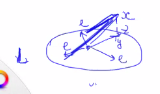
\includegraphics[width=150px]{pic14} \\
		длина любой наклонной больше, чем длина перпендикуляра
	\end{theorem}
	\begin{proof}
		$\pu l \in L \; \; l\neq y \; \; \; \; \ \; \; \; \|x-l\|^2 = \|\underbrace{x - y}_{= z \in L^\perp} + \underbrace{y - e}_{\in L} \|^2 \underset{\text{по т. Пифагора}}{=} ||x-y||^2 + \underset{>0 \; \; y\neq l}{||y-l||^2} \n
		\Rightarrow ||x-l||^2 > ||x-y||^2 \Rightarrow$ все.
	\end{proof}
	\begin{defin}
		$dist (x, L) = \min\limits_{l \in L} \|x-l\| = \underset{\text{расстояние от }x \text{ до } L}{\| x - y\| = \|z\|}$
	\end{defin}
\end{document}